\documentclass[a4paper,12pt]{article}

\usepackage[utf8]{inputenc}
\usepackage[spanish]{babel}
\usepackage{amsmath, amssymb}
\usepackage{graphicx}
\usepackage{float}
\usepackage{booktabs}
\usepackage{xcolor}
\usepackage{listings}
\usepackage{caption}
\usepackage{fancyhdr}
\usepackage{hyperref}
\usepackage{tikz}

\hypersetup{
    colorlinks=true,
    linkcolor=blue,
    urlcolor=blue,
    pdftitle={Práctica 1 - ZedBoard},
}

% === Definición de colores similares a Vivado ===
\definecolor{vivadoKeyword}{rgb}{0.6,0.0,0.6}
\definecolor{vivadoComment}{rgb}{0.0,0.5,0.0}
\definecolor{vivadoString}{rgb}{0.5,0.2,0.0}
\definecolor{vivadoBackground}{rgb}{0.97,0.97,0.97}

\lstdefinelanguage{VHDL}{
    morekeywords={library, use, entity, is, port, in, out, end, architecture, of, begin, signal, if, then, else, when, others, xor, and, or, not},
    sensitive=true,
    morecomment=[l]--,
    morestring=[b]",
}

\lstset{
    language=VHDL,
    backgroundcolor=\color{vivadoBackground},
    keywordstyle=\color{vivadoKeyword}\bfseries,
    commentstyle=\color{vivadoComment}\itshape,
    stringstyle=\color{vivadoString},
    basicstyle=\ttfamily\small,
    numbers=left,
    numberstyle=\tiny,
    numbersep=5pt,
    frame=single,
    breaklines=true,
    tabsize=2,
    captionpos=b
}

\title{Práctica N°1: Inicializacion de OLED en la placa ZedBoard}
\date{}

\begin{document}
\maketitle
\tableofcontents
\newpage

\section{Objetivos de la práctica}
\label{sec:objetivos}

\subsection{Objetivo general}
Implementar un sistema completo en la tarjeta ZedBoard para el control de una pantalla OLED mediante descripciones en VHDL, integrando módulos de inicialización, temporización y comunicación SPI, con el fin de comprender el flujo de diseño digital en Vivado y la interacción hardware–software en un entorno FPGA.

\subsection{Objetivos específicos}
\begin{itemize}
  \item Reconocer las características técnicas de la ZedBoard relevantes para el manejo de periféricos externos.
  \item Configurar el arranque de la tarjeta mediante memoria SD, verificando el proceso de carga en la terminal serie.
  \item Desarrollar y analizar los bloques VHDL de soporte: \texttt{ascii\_rom}, \texttt{delay}, \texttt{spi\_ctrl}, \texttt{oled\_init}, \texttt{oled\_ex} y \texttt{oled\_ctrl}.
  \item Asignar correctamente los pines físicos del FPGA para garantizar la comunicación con la pantalla OLED en los niveles de tensión adecuados.
  \item Validar el funcionamiento del sistema en placa mostrando el alfabeto y el mensaje \emph{"Hello World!"} en la pantalla OLED.
\end{itemize}


\section{Reconocimiento de las características de la ZedBoard (Zynq-7000 XC7Z020)}
\label{sec:zedboard_caracteristicas}

\subsection{Resumen de la plataforma}
La ZedBoard es una tarjeta de evaluación basada en el SoC Xilinx Zynq--7000 \textbf{XC7Z020-1CLG484C}, que integra un \emph{Processing System} (PS) con doble \textit{ARM Cortex-A9} y lógica programable \emph{7-Series} (\(m\)85\,k celdas lógicas), más un conjunto robusto de periféricos y cabezales de expansión.

\begin{itemize}
  \item \textbf{SoC}: Zynq XC7Z020 (PS + PL). Configuración primaria desde \emph{QSPI Flash}. Alternativas: \emph{JTAG} en cascada e \emph{SD Card}.
  \item \textbf{Memoria a bordo}: {512}{MB} DDR3 (128M\(\times\)16 \(\times 2\), bus de 32\,bits), {256}{Mb} \emph{Quad-SPI} Flash. 
  \item \textbf{Display/Audio}: HDMI (ADV7511), VGA 12-bit (R,G,B por R-2R), OLED 128\(\times\)32 (UG-2832HSWEG04), códec I\textsuperscript{2}S ADAU1761 (entrada/salida estéreo, 8–96\,kHz). 
  \item \textbf{USB}: USB-JTAG integrado (SMT1-equivalente), USB-UART (CY7C64225), USB OTG (TUSB1210, \emph{ver nota de compatibilidad}).
  \item \textbf{Red}: PHY Gigabit Ethernet 88E1518 vía RGMII, con RJ45 de magnetismo integrado. 
  \item \textbf{Expansión}: 1x FMC LPC (Vadj seleccionable), 5x Pmod (4 para PL, 1 para PS/MIO), con protección ESD en líneas de datos. 
  \item \textbf{Relojes}: {33.333}{MHz} (PS) y {100}{MHz} (PL). 
  \item \textbf{E/S de usuario}: 7 botones (5 PL, 2 PS), 8 \emph{slide switches} (PL), 9 LEDs de usuario (8 PL, 1 PS), LED DONE (PL). 
  \item \textbf{Alimentación}: Entrada {12}{V} @ {5}{A} (jack 5.5/2.5\,mm, centro positivo), con reguladores y secuenciación acorde a Zynq; LED \emph{Power Good}. 
\end{itemize}

\paragraph{Nota crítica (USB OTG).}
Tras el diseño, se reportó una incompatibilidad temporal de temporización entre el PHY TUSB1210 y Zynq; no se recomienda en diseños nuevos—revisar errata del fabricante para detalles y mitigaciones.

\paragraph{Referencia Visual de la placa.}
De manera adicional se incluye una imagen referencial del dispositivo en el que se enlistan los distintos puertos disponibles.

\begin{center}
    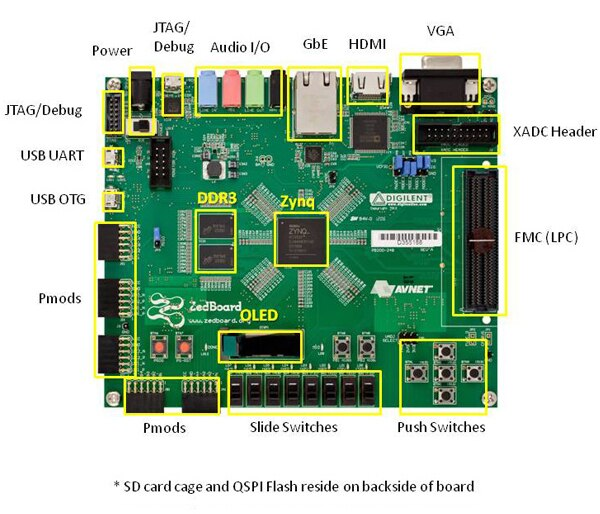
\includegraphics[width=0.7\linewidth]{ZedBoard/placa.png}
\end{center}
\textbf{Placa de desarrollo ZedBoard (Zynq-7000 XC7Z020) }

\subsection{Asignación de bancos y voltajes}
El encapsulado CLG484 organiza los bancos PS/PL según la Fig.~\ref{fig:banks} (ver guía). Los voltajes por banco en ZedBoard son los de la Tabla~\ref{tab:bank_voltages}. 

\begin{table}[H]
\centering
\caption{Voltajes por banco (ZedBoard).}
\label{tab:bank_voltages}
\begin{tabular}{lll}
\toprule
\textbf{Sección} & \textbf{Banco} & \textbf{Voltaje (por defecto)} \\
\midrule
PS (MIO)      & MIO 0/500 & 3.3\,V \\
              & MIO 1/501 & 1.8\,V \\
DDR           & DDR       & 1.5\,V \\
\midrule
PL            & Bank 0    & 3.3\,V \\
              & Bank 13   & 3.3\,V \\
              & Bank 33   & 3.3\,V \\
              & Bank 34   & Vadj (2.5\,V por defecto) \\
              & Bank 35   & Vadj (2.5\,V por defecto) \\
\bottomrule
\end{tabular}
\end{table}

\paragraph{Advertencia Vadj (FMC).} \emph{Jumper} J18 selecciona Vadj (1.8/2.5/3.3\,V). Por seguridad, 3.3\,V no viene poblado para no dañar \emph{mezzanines} FMC que sólo admiten 1.8/2.5\,V. Verifica \textbf{siempre} J18 antes de conectar una tarjeta FMC.

\subsection{Memoria del sistema}
\textbf{DDR3}: 2\(\times\) Micron 128\,M\(\times\)16 (\(x32\) total) = {512}{MB}, con controlador/PHY duros en PS. Velocidades hasta {533}{MHz} (1066\,MT/s). Tensión 1.5\,V, terminación VTT 0.75\,V, VREF=0.5\(\times\)VDDQ.

\textbf{QSPI Flash}: Spansion S25FL256S {256}{Mb}, x1/x2/x4, hasta {104}{MHz}; interfaz por MIO[1:6,8] (feedback en MIO[8]) y \emph{primary boot}. 

\textbf{SD}: Interfaz SD0 PS por MIO[40–47]; traslación de nivel vía TXS02612 (la ranura es 3.3\,V, MIO 1.8\,V). 

\subsection{Interfaces de visualización y audio}
\textbf{HDMI}: ADV7511 (225\,MHz, HDMI 1.4/DVI 1.0, hasta 1080p60, YCbCr 4:2:2 de 16\,bit). 

\textbf{VGA}: 12\,bits (4\,bits por color desde PL mediante red resistiva). 

\textbf{OLED}: UG-2832HSWEG04 128\(\times\)32 mono; interfaz SPI (CS\#, RES\#, D/C\#, SCLK, SDIN) y pines de potencia/booster (VBAT, VCC, etc.). 

\textbf{Audio}: ADAU1761 (I\textsuperscript{2}S), 8–96\,kHz, control por I\textsuperscript{2}C, \emph{line/mic in}, \emph{line/headphone out}. 

\subsection{USB, UART y JTAG}
\textbf{USB OTG}: TUSB1210 por ULPI \(\rightarrow\) MIO[28–39]; ver nota de compatibilidad. 

\textbf{USB–UART}: CY7C64225 con traslación TXS0102; PS UART1 por MIO[48–49] (1.8\,V \(\leftrightarrow\) 3.3\,V). 

\textbf{USB–JTAG}: Módulo Digilent SMT1–equivalente, plenamente soportado por Vivado/SDK. 

\subsection{Red Ethernet}
PHY Gigabit 88E1518 (RGMII sobre MIO 1/501 a 1.8\,V, con PS\_MIO\_VREF=0.9\,V). Conector RJ45 con magnetismo y LEDs de estado. 

\subsection{E/S de usuario}
\textbf{Botones}: 5 PL (BTNU/BTND/BTNL/BTNR/BTNC), 2 PS (PB1/PB2, MIO50/51). 

\textbf{Switches}: 8 \emph{slide switches} (SW0–SW7) hacia PL, polarizados mediante resistores a Vadj/GND. 

\textbf{LEDs}: 8 PL (LD0–LD7, activos en alto, limitación 390\,\(\Omega\)), 1 PS (LD9, MIO7). 

\subsection{Conectores de expansión}
\textbf{FMC LPC}: Bancos 34/35 con Vadj seleccionable (1.8/2.5/3.3\,V); CC/MRCC según guía, restricciones de \emph{skew} e impedancia; \textbf{verifica J18} antes de acoplar.

\textbf{Pmod (2x6)}: 5 conectores (4 en PL, 1 PS/MIO[0,9–15]); pares diferenciales en JC1/JD1 para LVDS hasta \(m\)525\,Mb/s; ESD en líneas de datos. 

\textbf{AMS (XADC)}: Cabecera analógica (VP/VN, VAUX0/8, DXP/DXN), filtros anti-\emph{aliasing}, VREF 1.25\,V y VCCADC 1.8\,V. 

\subsection{Reloj y reset}
\textbf{Relojes}: {33.333}{MHz} (PS) y {100}{MHz} (PL, GC pin en Bank 13). 

\textbf{Resets}: \emph{PS\_POR\_B} (monitorea regulación de fuentes), \emph{PROG\_B} (BTN6, reinicia PL), \emph{PS\_RST/BTN7} (reset del sistema sin re-muestrear modo de arranque). 

\subsection{Modos de configuración/arranque}
Selección por \emph{mode pins} MIO[6:2]: \textbf{SD Card} por defecto (JP8–JP10 = 110), \emph{QSPI}, \emph{JTAG}; JP11 decide uso de PLL internos. MIO[2] define \emph{JTAG cascaded} (0) o independiente (1). 

\subsection{Alimentación y consumo}
Entrada primaria {12}{V} (jack 5.5/2.5\,mm, {4}{A}–{5}{A}); protección, \emph{current shunt} {10}{m$\Omega$} (medición en J21), secuenciación conforme a Zynq (Vccint \(\rightarrow\) Vccaux \(\rightarrow\) Vcco/Vadj \(\rightarrow\) DDR/VTT), LED \emph{Power Good}. Tabla de corrientes estimadas disponible en la guía (p.ej., PS/PL, DDR, periféricos).

\subsection{Jumper relevantes (por defecto)}
\begin{itemize}
  \item \textbf{JP6}: Pull-down en PS\_MIO0 (requerido para boot SD en silicio CES). 
  \item \textbf{JP7–JP11}: \emph{Boot Mode} y PLL (SD por defecto; PLL usado). 
  \item \textbf{J18}: Selección Vadj (1.8\,V por defecto). 
\end{itemize}
Consulta el mapa de jumpers de la placa para posiciones exactas. 

\section{Arranque desde microSD (ZedBoard)}
\subsection*{1) ¿Cuál es el modo de arrancar la placa usando una SD?}
\begin{enumerate}
  \item \textbf{La ZedBoard arranca por defecto desde microSD} (el PS lee los \emph{mode pins} MIO[8:2] y selecciona SD como dispositivo primario). 
  \item Inserta una microSD (Clase 4+). La interfaz SD0 del PS usa MIO[40--47] y un traductor TXS02612 (3.3\,V $\leftrightarrow$ 1.8\,V), con \textbf{JP6 en corto para habilitar SD}. 
  \item Formatea en \textbf{FAT32} y coloca en la raíz los archivos de arranque (\texttt{BOOT.BIN} y, si usas Linux, \texttt{boot.scr}/\texttt{image.ub}). La SD sirve tanto para \emph{boot} como para almacenamiento. 
  \item Enciende la placa. (Si tu diseño requiere configurar la PL al inicio, incluye el \texttt{.bit} dentro de \texttt{BOOT.BIN} para que el FSBL lo cargue).
\end{enumerate}

\subsection*{2) ¿Cómo se ve el proceso en la terminal COM?}
\begin{enumerate}
  \item Conecta el \textbf{USB--UART} en \textbf{J14}. Este puente (CY7C64225) expone el \textbf{UART1 del PS} por MIO[48:49] mediante un \emph{level shifter} TXS0102. 
  \item Abre un terminal serial (p.\,ej., TeraTerm/Putty) en el puerto COM enumerado. Verás mensajes del \textbf{FSBL/U-Boot/Linux} durante el \emph{boot}. (La velocidad típica de imágenes de referencia es 115200\,8N1; usa la que defina tu \emph{build}).
\end{enumerate}

\subsection*{3) ¿Cómo cargar otra imagen Linux (cambiar el programa de la SD)?}
\begin{enumerate}
  \item Apaga la placa y retira la microSD.
  \item En la partición \textbf{FAT32}, reemplaza los ficheros según tu \emph{flow}:
  \begin{itemize}
    \item \textbf{Mínimo}: \texttt{BOOT.BIN} (FSBL + U-Boot; opcionalmente el \texttt{.bit} si quieres configurar PL al inicio).
    \item \textbf{Arranque directo}: \texttt{boot.scr} (script de U-Boot) y \texttt{image.ub} (kernel+dtb+initramfs) u \texttt{Image}/\texttt{system.dtb}/rootfs. 
  \end{itemize}
  \item Inserta la SD y enciende. El PS \textbf{bootea desde SD} y ejecuta lo nuevo sin usar JTAG. 
\end{enumerate}

\section{Descripción del codigo}

\subsection{ROM de fuente ASCII (ascii\_rom.vhd)}
\label{sec:ascii_rom}

\subsubsection*{Código fuente}
\begin{lstlisting}[language=VHDL,basicstyle=\ttfamily\small,frame=single,caption={ascii\_rom.vhd}]
-- Description: ROM containing ASCII character data.

library ieee;
use ieee.std_logic_1164.all;
use ieee.std_logic_arith.all;
use ieee.std_logic_unsigned.all;

entity ascii_rom is
    port (  clk     : in std_logic; -- System clock
            addr    : in std_logic_vector (10 downto 0); -- Memory address
            dout    : out std_logic_vector (7 downto 0)); -- Data from memory
end ascii_rom;

architecture behavioral of ascii_rom is

    -- 1024 elements, 8 bits each
    type memory is array (0 to 1023) of std_logic_vector (7 downto 0);

    -- ASCII character data
    constant rom_data : memory := ( x"00", x"00", x"00", x"00", x"00", x"00", x"00", x"00",
    x"00", x"00", x"00", x"00", x"00", x"00", x"00", x"00",
    x"00", x"00", x"00", x"00", x"00", x"00", x"00", x"00",
    x"00", x"00", x"00", x"00", x"00", x"00", x"00", x"00",
    x"00", x"00", x"00", x"00", x"00", x"00", x"00", x"00",
    x"00", x"00", x"00", x"00", x"00", x"00", x"00", x"00",
    x"00", x"00", x"00", x"00", x"00", x"00", x"00", x"00",
    x"00", x"00", x"00", x"00", x"00", x"00", x"00", x"00",
    x"00", x"00", x"00", x"00", x"00", x"00", x"00", x"00",
    x"00", x"00", x"00", x"00", x"00", x"00", x"00", x"00",
    x"00", x"00", x"00", x"00", x"00", x"00", x"00", x"00",
    x"00", x"00", x"00", x"00", x"00", x"00", x"00", x"00",
    x"00", x"00", x"00", x"00", x"00", x"00", x"00", x"00",
    x"00", x"00", x"00", x"00", x"00", x"00", x"00", x"00",
    x"00", x"00", x"00", x"00", x"00", x"00", x"00", x"00",
    x"00", x"00", x"00", x"00", x"00", x"00", x"00", x"00",
    x"00", x"00", x"00", x"00", x"00", x"00", x"00", x"00",
    x"00", x"00", x"00", x"00", x"00", x"00", x"00", x"00",
    x"00", x"00", x"00", x"00", x"00", x"00", x"00", x"00",
    x"00", x"00", x"00", x"00", x"00", x"00", x"00", x"00",
    x"00", x"00", x"00", x"00", x"00", x"00", x"00", x"00",
    x"00", x"00", x"00", x"00", x"00", x"00", x"00", x"00",
    x"00", x"00", x"00", x"00", x"00", x"00", x"00", x"00",
    x"00", x"00", x"00", x"00", x"00", x"00", x"00", x"00",
    x"00", x"00", x"00", x"00", x"00", x"00", x"00", x"00",
    x"00", x"00", x"00", x"00", x"00", x"00", x"00", x"00",
    x"00", x"00", x"00", x"00", x"00", x"00", x"00", x"00",
    x"00", x"00", x"00", x"00", x"00", x"00", x"00", x"00",
    x"00", x"00", x"00", x"00", x"00", x"00", x"00", x"00",
    x"00", x"00", x"00", x"00", x"00", x"00", x"00", x"00",
    x"00", x"00", x"00", x"00", x"00", x"00", x"00", x"00",
    x"00", x"00", x"00", x"00", x"00", x"00", x"00", x"00",
    x"00", x"00", x"00", x"5f", x"00", x"00", x"00", x"00",
    x"00", x"00", x"03", x"00", x"03", x"00", x"00", x"00",
    x"64", x"3c", x"26", x"64", x"3c", x"26", x"24", x"00",
    x"26", x"49", x"49", x"7f", x"49", x"49", x"32", x"00",
    x"42", x"25", x"12", x"08", x"24", x"52", x"21", x"00",
    x"20", x"50", x"4e", x"55", x"22", x"58", x"28", x"00",
    x"00", x"00", x"00", x"03", x"00", x"00", x"00", x"00",
    x"00", x"00", x"1c", x"22", x"41", x"00", x"00", x"00",
    x"00", x"00", x"00", x"41", x"22", x"1c", x"00", x"00",
    x"00", x"15", x"15", x"0e", x"0e", x"15", x"15", x"00",
    x"00", x"08", x"08", x"3e", x"08", x"08", x"00", x"00",
    x"00", x"00", x"00", x"50", x"30", x"00", x"00", x"00",
    x"00", x"08", x"08", x"08", x"08", x"08", x"00", x"00",
    x"00", x"00", x"00", x"40", x"00", x"00", x"00", x"00",
    x"40", x"20", x"10", x"08", x"04", x"02", x"01", x"00",
    x"00", x"3e", x"41", x"41", x"41", x"3e", x"00", x"00",
    x"00", x"00", x"41", x"7f", x"40", x"00", x"00", x"00",
    x"00", x"42", x"61", x"51", x"49", x"6e", x"00", x"00",
    x"00", x"22", x"41", x"49", x"49", x"36", x"00", x"00",
    x"00", x"18", x"14", x"12", x"7f", x"10", x"00", x"00",
    x"00", x"27", x"49", x"49", x"49", x"71", x"00", x"00",
    x"00", x"3c", x"4a", x"49", x"48", x"70", x"00", x"00",
    x"00", x"43", x"21", x"11", x"0d", x"03", x"00", x"00",
    x"00", x"36", x"49", x"49", x"49", x"36", x"00", x"00",
    x"00", x"06", x"09", x"49", x"29", x"1e", x"00", x"00",
    x"00", x"00", x"00", x"12", x"00", x"00", x"00", x"00",
    x"00", x"00", x"00", x"52", x"30", x"00", x"00", x"00",
    x"00", x"00", x"08", x"14", x"14", x"22", x"00", x"00",
    x"00", x"14", x"14", x"14", x"14", x"14", x"14", x"00",
    x"00", x"00", x"22", x"14", x"14", x"08", x"00", x"00",
    x"00", x"02", x"01", x"59", x"05", x"02", x"00", x"00",
    x"3e", x"41", x"5d", x"55", x"4d", x"51", x"2e", x"00",
    x"40", x"7c", x"4a", x"09", x"4a", x"7c", x"40", x"00",
    x"41", x"7f", x"49", x"49", x"49", x"49", x"36", x"00",
    x"1c", x"22", x"41", x"41", x"41", x"41", x"22", x"00",
    x"41", x"7f", x"41", x"41", x"41", x"22", x"1c", x"00",
    x"41", x"7f", x"49", x"49", x"5d", x"41", x"63", x"00",
    x"41", x"7f", x"49", x"09", x"1d", x"01", x"03", x"00",
    x"1c", x"22", x"41", x"49", x"49", x"3a", x"08", x"00",
    x"41", x"7f", x"08", x"08", x"08", x"7f", x"41", x"00",
    x"00", x"41", x"41", x"7F", x"41", x"41", x"00", x"00",
    x"30", x"40", x"41", x"41", x"3F", x"01", x"01", x"00",
    x"41", x"7f", x"08", x"0c", x"12", x"61", x"41", x"00",
    x"41", x"7f", x"41", x"40", x"40", x"40", x"60", x"00",
    x"41", x"7f", x"42", x"0c", x"42", x"7f", x"41", x"00",
    x"41", x"7f", x"42", x"0c", x"11", x"7f", x"01", x"00",
    x"1c", x"22", x"41", x"41", x"41", x"22", x"1c", x"00",
    x"41", x"7f", x"49", x"09", x"09", x"09", x"06", x"00",
    x"0c", x"12", x"21", x"21", x"61", x"52", x"4c", x"00",
    x"41", x"7f", x"09", x"09", x"19", x"69", x"46", x"00",
    x"66", x"49", x"49", x"49", x"49", x"49", x"33", x"00",
    x"03", x"01", x"41", x"7f", x"41", x"01", x"03", x"00",
    x"01", x"3f", x"41", x"40", x"41", x"3f", x"01", x"00",
    x"01", x"0f", x"31", x"40", x"31", x"0f", x"01", x"00",
    x"01", x"1f", x"61", x"14", x"61", x"1f", x"01", x"00",
    x"41", x"41", x"36", x"08", x"36", x"41", x"41", x"00",
    x"01", x"03", x"44", x"78", x"44", x"03", x"01", x"00",
    x"43", x"61", x"51", x"49", x"45", x"43", x"61", x"00",
    x"00", x"00", x"7f", x"41", x"41", x"00", x"00", x"00",
    x"01", x"02", x"04", x"08", x"10", x"20", x"40", x"00",
    x"00", x"00", x"41", x"41", x"7f", x"00", x"00", x"00",
    x"00", x"04", x"02", x"01", x"01", x"02", x"04", x"00",
    x"00", x"40", x"40", x"40", x"40", x"40", x"40", x"00",
    x"00", x"01", x"02", x"00", x"00", x"00", x"00", x"00",
    x"00", x"34", x"4a", x"4a", x"4a", x"3c", x"40", x"00",
    x"00", x"41", x"3f", x"48", x"48", x"48", x"30", x"00",
    x"00", x"3c", x"42", x"42", x"42", x"24", x"00", x"00",
    x"00", x"30", x"48", x"48", x"49", x"3f", x"40", x"00",
    x"00", x"3c", x"4a", x"4a", x"4a", x"2c", x"00", x"00",
    x"00", x"00", x"48", x"7e", x"49", x"09", x"00", x"00",
    x"00", x"26", x"49", x"49", x"49", x"3f", x"01", x"00",
    x"41", x"7f", x"48", x"04", x"44", x"78", x"40", x"00",
    x"00", x"00", x"44", x"7d", x"40", x"00", x"00", x"00",
    x"00", x"00", x"40", x"44", x"3d", x"00", x"00", x"00",
    x"41", x"7f", x"10", x"18", x"24", x"42", x"42", x"00",
    x"00", x"40", x"41", x"7f", x"40", x"40", x"00", x"00",
    x"42", x"7e", x"02", x"7c", x"02", x"7e", x"40", x"00",
    x"42", x"7e", x"44", x"02", x"42", x"7c", x"40", x"00",
    x"00", x"3c", x"42", x"42", x"42", x"3c", x"00", x"00",
    x"00", x"41", x"7f", x"49", x"09", x"09", x"06", x"00",
    x"00", x"06", x"09", x"09", x"49", x"7f", x"41", x"00",
    x"00", x"42", x"7e", x"44", x"02", x"02", x"04", x"00",
    x"00", x"64", x"4a", x"4a", x"4a", x"36", x"00", x"00",
    x"00", x"04", x"3f", x"44", x"44", x"20", x"00", x"00",
    x"00", x"02", x"3e", x"40", x"40", x"22", x"7e", x"40",
    x"02", x"0e", x"32", x"40", x"32", x"0e", x"02", x"00",
    x"02", x"1e", x"62", x"18", x"62", x"1e", x"02", x"00",
    x"42", x"62", x"14", x"08", x"14", x"62", x"42", x"00",
    x"01", x"43", x"45", x"38", x"05", x"03", x"01", x"00",
    x"00", x"46", x"62", x"52", x"4a", x"46", x"62", x"00",
    x"00", x"00", x"08", x"36", x"41", x"00", x"00", x"00",
    x"00", x"00", x"00", x"7f", x"00", x"00", x"00", x"00",
    x"00", x"00", x"00", x"41", x"36", x"08", x"00", x"00",
    x"00", x"18", x"08", x"08", x"10", x"10", x"18", x"00",
    x"AA", x"55", x"AA", x"55", x"AA", x"55", x"AA", x"55");

begin

    process (clk)
    begin
        if rising_edge(clk) then
            dout <= rom_data(conv_integer(addr));
        end if;
    end process;

end behavioral;
\end{lstlisting}

\subsubsection*{Lectura guiada y consideraciones de integración}
\begin{itemize}
  \item \textbf{Interfaz}:
  \begin{itemize}
    \item \texttt{clk}: lectura \emph{síncrona}; la salida \texttt{dout} se actualiza en flanco ascendente.
    \item \texttt{addr(10 downto 0)}: dirección de 11 bits. La ROM tiene 1024 ubicaciones (0..1023); por tanto, \textbf{usa sólo 10 bits efectivos} o garantiza que \texttt{addr(10)} siempre sea ‘0’ para evitar accesos fuera de rango.
    \item \texttt{dout(7 downto 0)}: byte de patrón de columna/fila del glifo (1 bpp).
  \end{itemize}

  \item \textbf{Organización de memoria}: 1024\,$\times$\,8 = 8192 bits (\(\approx\)8\,Kb). En 7-Series suele inferir 1 bloque \texttt{RAMB18E1} (o LUT ROM si el sintetizador decide). Con salida registrada, se cumple un timing cómodo para relojes de sistema comunes (50–100\,MHz).

  \item \textbf{Estilo y librerías}:
  \begin{itemize}
    \item Se usando \texttt{std\_logic\_arith} y \texttt{std\_logic\_unsigned} + \texttt{conv\_integer}. Son extensiones no estándar pero muy usadas. 
    \item \texttt{conv\_integer(addr)} asume que \texttt{addr} es un vector sin ‘X/Z’;
  \end{itemize}

  \item \textbf{Mapeo típico de glifos} :
  \[
    \text{addr} = \text{(código\_ASCII)} \times 8 \;+\; \text{fila\_de\_columna}
  \]
  con \(\text{fila\_de\_columna}\in[0,7]\) si el glifo es 8\(\times\)8. Se debe ajustar si la fuente es 5\(\times\)8 u otra variante. Ademas se aconseja verificar también si el bit menos significativo representa píxel “arriba” o “abajo”.
\end{itemize}

\subsection{Temporizador por milisegundos (delay.vhd)}
\label{sec:delay_ms}

\subsubsection*{Código fuente}

\begin{lstlisting}[language=VHDL,basicstyle=\ttfamily\small,frame=single,caption={delay.vhd}]

-- Description: Creates a delay of delay_ms ms.
--

library ieee;
use ieee.std_logic_1164.all;
use ieee.std_logic_arith.all;
use ieee.std_logic_unsigned.all;

entity delay is
    port (  clk         : in std_logic; -- System clock
            rst         : in std_logic;  -- Global synchronous reset
            delay_ms    : in std_logic_vector (11 downto 0); -- Amount of ms to delay
            delay_en    : in std_logic; -- Delay enable
            delay_fin   : out std_logic); -- Delay finish flag
end delay;

architecture behavioral of delay is

    type states is (Idle, Hold, Done);

    signal current_state : states := Idle; -- Signal for state machine
    signal clk_counter : std_logic_vector(16 downto 0) := (others => '0'); -- Counts up on every rising edge of clk
    signal ms_counter : std_logic_vector (11 downto 0) := (others => '0'); -- Counts up when clk_counter = 100,000

begin
    -- delay_fin goes high when delay is done
    delay_fin <= '1' when (current_state = Done and delay_en = '1') else '0';

    -- State machine for Delay block
    state_machine : process (clk)
    begin
        if rising_edge(clk) then
            if rst = '1' then -- When rst is asserted switch to Idle (synchronous)
                current_state <= Idle;
            else
                case current_state is
                    when Idle =>
                        if delay_en = '1' then -- Start delay on delay_en
                            current_state <= Hold;
                        end if;
                    when Hold =>
                        if ms_counter = delay_ms then -- Stay until delay_ms has occured
                            current_state <= Done;
                        end if;
                    when Done =>
                        if delay_en = '0' then -- Wait until delay_en is deasserted to go to Idle
                            current_state <= Idle;
                        end if;
                    when others =>
                        current_state <= Idle;
                end case;
            end if;
        end if;
    end process state_machine;
    -- Creates ms_counter that counts at 1KHz
    clk_div : process (clk)
    begin
        if rising_edge(clk) then
            if current_state = Hold then
                if clk_counter = "11000011010100000" then -- 100,000
                    clk_counter <= (others => '0');
                    ms_counter <= ms_counter + 1; -- Increments at 1KHz
                else
                    clk_counter <= clk_counter + 1;
                end if;
            else -- If not in the hold state reset counters
                clk_counter <= (others => '0');
                ms_counter <= (others => '0');
            end if;
        end if;
    end process;

end behavioral;
\end{lstlisting}

\subsubsection*{Lectura guiada y criterios de integración}
\begin{itemize}
  \item \textbf{Propósito}. Se implementa un retardo programable en milisegundos mediante una FSM con tres estados:
  \emph{Idle} (espera), \emph{Hold} (conteo) y \emph{Done} (finalización mediante \texttt{delay\_fin}).
  \item \textbf{Suposición de reloj}. El umbral \texttt{100000} implica {100}{MHz} de \texttt{clk} ({1}{ms} = 100\,000 ciclos). Si \texttt{clk} difiere, se debe ajustar el umbral o parametrizarlo.
  \item \textbf{Rango}. \texttt{delay\_ms} y \texttt{ms\_counter} son de 12 bits \(\Rightarrow\) hasta 4095\,ms (\(\approx\)4.095\,s).
  \item \textbf{Bandera de fin}. \texttt{delay\_fin} permanece en ‘1’ mientras el estado sea \emph{Done} y \texttt{delay\_en} siga en ‘1’. Cuando \texttt{delay\_en} cae a ‘0’, el módulo vuelve a \emph{Idle}.
  \item \textbf{Entradas dinámicas}. Si \texttt{delay\_ms} cambia durante \emph{Hold}, el objetivo se mueve; para comportamiento determinista se debe capturar \texttt{delay\_ms} al entrar en \emph{Hold}.
  \item \textbf{Sincronización}. \texttt{delay\_en} debe estar sincronizada a \texttt{clk}; si proviene de otro dominio o de un botón, se deben usar dos FF de sincronía y, si aplica, antirrebote.
  \item \textbf{Anchos de contador}. \texttt{clk\_counter} (17 bits) cubre 100\,000 correctamente (\(2^{17}=131{,}072\)).
  \item \textbf{Uso típico con OLED}. En secuencias de \emph{power-on} y comandos sensibles, se debe: programar \texttt{delay\_ms} \(\to\) poner \texttt{delay\_en}=1 \(\to\) esperar \texttt{delay\_fin} \(\to\) avanzar de estado.
\end{itemize}

\newpage


\subsection{Controlador SPI para OLED (spi_ctrl.vhd)}
\label{sec:spi_ctrl}

\subsubsection*{Código fuente}
\begin{lstlisting}[language=VHDL,basicstyle=\ttfamily\small,frame=single,caption={spi\_ctrl.vhd}]
--
-- Written by Ryan Kim, Digilent Inc.
-- Modified by Michael Mattioli
--
-- Description: SPI block that sends SPI data formatted oled_sclk active low with sdout changing
-- on the falling edge.
--

library ieee;
use ieee.std_logic_1164.all;
use ieee.std_logic_arith.all;
use ieee.std_logic_unsigned.all;

entity spi_ctrl is
    Port ( clk          : in std_logic; -- System clok (100MHz)
           rst          : in std_logic; -- Global synchronous reset
           en           : in std_logic; -- Block enable pin
           sdata        : in std_logic_vector (7 downto 0); -- Byte to be sent
           sdout        : out std_logic; -- Serial data out
           oled_sclk    : out std_logic; -- OLED serial clock
           fin          : out std_logic); -- Finish flag for block
end spi_ctrl;

architecture behavioral of spi_ctrl is

    type states is (Idle, Send, Done);

    signal current_state : states := Idle; -- Signal for state machine

    signal shift_register   : std_logic_vector (7 downto 0); -- Shift register to shift out sdata saved when en was set
    signal shift_counter    : std_logic_vector (3 downto 0); -- Keeps track how many bits were sent
    signal clk_divided      : std_logic := '1'; -- Used as oled_sclk
    signal counter          : std_logic_vector (4 downto 0) := (others => '0'); -- Count clocks to be used to divide clk
    signal temp_sdata       : std_logic := '1'; -- Tied to sdout

    signal falling : std_logic := '0'; -- Signal indicating that the clk has just fell

begin

    clk_divided <= not counter(4); -- oled_sclk = clk / 32
    oled_sclk <= clk_divided;
    sdout <= temp_sdata;
    fin <= '1' when current_state = Done else '0';

    state_machine : process (clk)
    begin
        if rising_edge(clk) then
            if rst = '1' then -- Synchronous rst
                current_state <= Idle;
            else
                case current_state is
                    when Idle => -- Wait for en to go high
                        if en = '1' then
                            current_state <= Send;
                        end if;
                    when Send => -- Start sending bits, transition out when all bits are sent and oled_sclk is high
                        if shift_counter = "1000" and falling = '0' then
                            current_state <= Done;
                        end if;
                    when Done => -- Finish SPI transimission wait for en to go low
                        if en = '0' then
                            current_state <= Idle;
                        end if;
                    when others =>
                        current_state <= Idle;
                end case;
            end if;
        end if;
    end process state_machine;

    clk_div : process (clk)
    begin
        if rising_edge(clk) then
            if current_state = Send then -- Start clock counter when in send state
                counter <= counter + 1;
            else -- Reset clock counter when not in send state
                counter <= (others => '0');
            end if;
        end if;
    end process clk_div;

    spi_send_byte : process (clk) -- Sends SPI data formatted oled_sclk active low with sdout changing on the falling edge
    begin
        if rising_edge(clk) then
            if current_state = Idle then
                shift_counter <= (others => '0');
                shift_register <= sdata; -- Keeps placing sdata into shift_register so that when state goes to send it has the latest sdata
                temp_sdata <= '1';
            elsif current_state = Send then
                if clk_divided = '0' and falling = '0' then -- If on the falling edge of clk_divided
                    falling <= '1'; -- Indicate that it is passed the falling edge
                    temp_sdata <= shift_register(7); -- Send out the MSB
                    shift_register <= shift_register(6 downto 0) & '0'; -- Shift through sdata
                    shift_counter <= shift_counter + 1; -- Keep track of what bit it is on
                elsif clk_divided = '1' then -- On oled_sclk high reset the falling flag
                    falling <= '0';
                end if;
            end if;
        end if;
    end process spi_send_byte;

end behavioral;
\end{lstlisting}

\subsubsection*{Lectura guiada y criterios de integración}
\begin{itemize}
  \item \textbf{Función y modo SPI}. El bloque envía un byte por SPI con \textbf{datos cambiando en el flanco de bajada} de \texttt{oled\_sclk} y, por tanto, se debe muestrear en el \textbf{flanco de subida}. Esto corresponde al modo habitual \textbf{CPOL=1, CPHA=1} (SPI modo 3) cuando la línea de reloj permanece en ‘1’ en reposo y las transiciones válidas ocurren alta\(\to\)baja para el cambio y baja\(\to\)alta para el muestreo.
  \item \textbf{Frecuencia de reloj SPI}. \texttt{oled\_sclk} se obtiene como \(\texttt{clk}/32\) usando \(\texttt{counter(4)}\). Con \(\texttt{clk}=100~\text{MHz}\), el reloj SPI nominal es \(\,100~\text{MHz}/32 = 3.125~\text{MHz}\).  
        Si se requiere otra velocidad, se debe ajustar el divisor (ancho del contador o bit usado).
  \item \textbf{Protocolo de envío}. En estado \emph{Send}, el MSB (\texttt{shift\_register(7)}) se presenta en \texttt{sdout} justo en cada flanco de bajada de \texttt{oled\_sclk} (\texttt{clk\_divided='0'} con \texttt{falling='0'}), luego se desplaza el registro y se incrementa \texttt{shift\_counter}. Tras 8 bits (\texttt{"1000"}) y con \texttt{oled\_sclk} en alto (\texttt{falling='0'}), se pasa a \emph{Done}.
  \item \textbf{Señales de control}.  
        \texttt{en} inicia la transacción; \texttt{fin} es de nivel alto en \emph{Done} hasta que \texttt{en} cae a ‘0’. Si se requiere un pulso de “fin”, se debe derivar un \emph{one-shot} sobre la transición \emph{Send}\(\to\)\emph{Done}.
  \item \textbf{Cargas e inactividad}. \texttt{sdout} queda en ‘1’ fuera de \emph{Send}; \texttt{clk\_divided} arranca en ‘1’. Si el periférico OLED exige \texttt{SCLK} inactivo alto y \texttt{SDOUT} en ‘1’, esta convención es compatible.
  \item \textbf{Interfaz superior}. La gestión de \texttt{CS\_n} y \texttt{DC} no está incluida en este bloque; se debe controlar desde la FSM superior (driver OLED) con temporización coherente: \texttt{CS\_n} activo antes del primer bit y liberado tras \emph{Done}, \texttt{DC} estable durante todo el byte.
  \item \textbf{Dominios y robustez}. \texttt{en} y \texttt{sdata} deben estar estables y sincronizados a \texttt{clk} al entrar en \emph{Send}. Si \texttt{sdata} puede cambiar, se debe amostrar en \emph{Idle} (ya contemplado por \texttt{shift\_register<=sdata}).
  \item \textbf{Casos límite}.  
        \begin{itemize}
          \item Si \texttt{en} cae antes de completar 8 bits, la FSM no aborta; finalizará y esperará \texttt{en}=‘0’ en \emph{Done}. La lógica superior debe mantener \texttt{en}=‘1’ durante toda la transferencia.
          \item Si se encadenan bytes, se debe mantener \texttt{en}=‘1’, monitorizar \texttt{fin} y cargar un nuevo \texttt{sdata} durante la ventana de \texttt{oled\_sclk} alto antes del siguiente flanco de bajada.
        \end{itemize}
\end{itemize}

\subsection{Secuencia de inicialización de la OLED (oled_init.vhd)}
\label{sec:oled_init}

\subsubsection*{Código fuente}
\begin{lstlisting}[language=VHDL,basicstyle=\ttfamily\small,frame=single,caption={oled\_init.vhd}]
--
-- Written by Ryan Kim, Digilent Inc.
-- Modified by Michael Mattioli
--
-- Description: Runs the initialization sequence for the OLED display.
--

library ieee;
use ieee.std_logic_1164.all;
use ieee.std_logic_arith.all;
use ieee.std_logic_unsigned.all;

entity oled_init is
    port (  clk         : in std_logic; -- System clock
            rst         : in std_logic; -- Global synchronous reset
            en          : in std_logic; -- Block enable pin
            sdout       : out std_logic; -- SPI data out
            oled_sclk   : out std_logic; -- SPI clock
            oled_dc     : out std_logic; -- Data/Command pin
            oled_res    : out std_logic; -- OLED reset
            oled_vbat   : out std_logic; -- oled_vbat enable
            oled_vdd    : out std_logic; -- oled_vdd enable
            fin         : out std_logic); -- Finish flag for block
end oled_init;

architecture behavioral of oled_init is

    component spi_ctrl
        port (  clk         : in std_logic;
                rst         : in std_logic;
                en          : in std_logic;
                sdata       : in std_logic_vector (7 downto 0);
                sdout       : out std_logic;
                oled_sclk   : out std_logic;
                fin         : out std_logic);
    end component;

    component delay
        port (  clk         : in std_logic;
                rst         : in std_logic;
                delay_ms    : in std_logic_vector (11 downto 0);
                delay_en    : in std_logic;
                delay_fin   : out std_logic);
    end component;

    type states is (Transition1,
                    Transition2,
                    Transition3,
                    Transition4,
                    Transition5,
                    Idle,
                    VddOn,
                    Wait1,
                    DispOff,
                    ResetOn,
                    Wait2,
                    ResetOff,
                    ChargePump1,
                    ChargePump2,
                    PreCharge1,
                    PreCharge2,
                    VbatOn,
                    Wait3,
                    DispContrast1,
                    DispContrast2,
                    InvertDisp1,
                    InvertDisp2,
                    ComConfig1,
                    ComConfig2,
                    DispOn,
                    FullDisp,
                    Done);

    signal current_state : states := Idle;
    signal after_state : states := Idle;

    signal temp_dc      : std_logic := '0';
    signal temp_res     : std_logic := '1';
    signal temp_vbat    : std_logic := '1';
    signal temp_vdd     : std_logic := '1';
    signal temp_fin     : std_logic := '0';

    signal temp_delay_ms    : std_logic_vector (11 downto 0) := (others => '0');
    signal temp_delay_en    : std_logic := '0';
    signal temp_delay_fin   : std_logic;
    signal temp_spi_en      : std_logic := '0';
    signal temp_sdata       : std_logic_vector (7 downto 0) := (others => '0');
    signal temp_spi_fin     : std_logic;

begin

    spi_comp: spi_ctrl port map (   clk => clk,
                                    rst => rst,
                                    en => temp_spi_en,
                                    sdata => temp_sdata,
                                    sdout => sdout,
                                    oled_sclk => oled_sclk,
                                    fin => temp_spi_fin);

    delay_comp: delay port map (clk => clk,
                                rst => rst,
                                delay_ms => temp_delay_ms,
                                delay_en => temp_delay_en,
                                delay_fin => temp_delay_fin);

    oled_dc <= temp_dc;
    oled_res <= temp_res;
    oled_vbat <= temp_vbat;
    oled_vdd <= temp_vdd;
    fin <= temp_fin;

    -- Delay 100 ms after VbatOn
    temp_delay_ms <=    "000001100100" when after_state = DispContrast1 else -- 100ms
                        "000000000001"; -- 1ms

    process (clk)
    begin
        if rising_edge(clk) then
            if rst = '1' then
                current_state <= Idle;
                temp_res <= '0';
            else
                temp_res <= '1';
                case current_state is
                    when Idle =>
                        if en = '1' then
                            temp_dc <= '0';
                            current_state <= VddOn;
                        end if;

                    -- Initialization Sequence
                    -- This should be done everytime the OLED display is started
                    when VddOn =>
                        temp_vdd <= '0';
                        current_state <= Wait1;
                    when Wait1 =>
                        after_state <= DispOff;
                        current_state <= Transition3;
                    when DispOff =>
                        temp_sdata <= "10101110"; -- 0xAE
                        after_state <= ResetOn;
                        current_state <= Transition1;
                    when ResetOn =>
                        temp_res <= '0';
                        current_state <= Wait2;
                    when Wait2 =>
                        after_state <= ResetOff;
                        current_state <= Transition3;
                    when ResetOff =>
                        temp_res <= '1';
                        after_state <= ChargePump1;
                        current_state <= Transition3;
                    when ChargePump1 =>
                        temp_sdata <= "10001101"; -- 0x8D
                        after_state <= ChargePump2;
                        current_state <= Transition1;
                    when ChargePump2 =>
                        temp_sdata <= "00010100"; -- 0x14
                        after_state <= PreCharge1;
                        current_state <= Transition1;
                    when PreCharge1  =>
                        temp_sdata <= "11011001"; -- 0xD9
                        after_state <= PreCharge2;
                        current_state <= Transition1;
                    when PreCharge2 =>
                        temp_sdata <= "11110001"; -- 0xF1
                        after_state <= VbatOn;
                        current_state <= Transition1;
                    when VbatOn =>
                        temp_vbat <= '0';
                        current_state <= Wait3;
                    when Wait3 =>
                        after_state <= DispContrast1;
                        current_state <= Transition3;
                    when DispContrast1=>
                        temp_sdata <= "10000001"; -- 0x81
                        after_state <= DispContrast2;
                        current_state <= Transition1;
                    when DispContrast2=>
                        temp_sdata <= "00001111"; -- 0x0F
                        after_state <= InvertDisp1;
                        current_state <= Transition1;
                    when InvertDisp1 =>
                        temp_sdata <= "10100000"; -- 0xA0
                        after_state <= InvertDisp2;
                        current_state <= Transition1;
                    when InvertDisp2 =>
                        temp_sdata <= "11000000"; -- 0xC0
                        after_state <= ComConfig1;
                        current_state <= Transition1;
                    when ComConfig1 =>
                        temp_sdata <= "11011010"; -- 0xDA
                        after_state <= ComConfig2;
                        current_state <= Transition1;
                    when ComConfig2 =>
                        temp_sdata <= "00000000"; -- 0x00
                        after_state <= DispOn;
                        current_state <= Transition1;
                    when DispOn =>
                        temp_sdata <= "10101111"; -- 0xAF
                        after_state <= Done;
                        current_state <= Transition1;
                    -- End Initialization sequence

                    -- Used for debugging, turns the entire screen on regardless of memory
                    when FullDisp =>
                        temp_sdata <= "10100101"; -- 0xA5
                        after_state <= Done;
                        current_state <= Transition1;

                    -- Done state
                    when Done =>
                        if en = '0' then
                            temp_fin <= '0';
                            current_state <= Idle;
                        else
                            temp_fin <= '1';
                        end if;

                    -- SPI transitions
                    -- 1. Set en to 1
                    -- 2. Waits for spi_ctrl to finish
                    -- 3. Goes to clear state (Transition5)
                    when Transition1 =>
                        temp_spi_en <= '1';
                        current_state <= Transition2;
                    when Transition2 =>
                        if temp_spi_fin = '1' then
                            current_state <= Transition5;
                        end if;
                    -- End SPI transitions

                    -- Delay transitions
                    -- 1. Set delay_en to 1
                    -- 2. Waits for delay to finish
                    -- 3. Goes to Clear state (Transition5)
                    when Transition3 =>
                        temp_delay_en <= '1';
                        current_state <= Transition4;
                    when Transition4 =>
                        if temp_delay_fin = '1' then
                            current_state <= Transition5;
                        end if;
                    -- End delay transitions

                    -- Clear transitions
                    -- 1. Sets both delay_en and en to 0
                    -- 2. Go to after state
                    when Transition5 =>
                        temp_spi_en <= '0';
                        temp_delay_en <= '0';
                        current_state <= after_state;
                    -- End Clear transitions

                    when others =>
                        current_state <= Idle;
                end case;
            end if;
        end if;
    end process;

end behavioral;
\end{lstlisting}

\subsubsection*{Lectura guiada y criterios de integración}
\begin{itemize}
  \item \textbf{Propósito general}. Se implementa una FSM que ejecuta la secuencia de arranque típica de un controlador tipo SSD1306: \texttt{DISPLAY\_OFF (0xAE)} \(\rightarrow\) pulso de \texttt{RESET} \(\rightarrow\) \texttt{CHARGE\_PUMP (0x8D,0x14)} \(\rightarrow\) \texttt{PRECHARGE (0xD9,0xF1)} \(\rightarrow\) habilitación de \texttt{VBAT} \(\rightarrow\) contraste \(\rightarrow\) mapeos \(\rightarrow\) \texttt{DISPLAY\_ON (0xAF)}.
  \item \textbf{Control de alimentación}. \texttt{oled\_vdd} y \texttt{oled\_vbat} se manejan como señales activas en nivel bajo (\texttt{'0'} = habilitado). Este mapeo debe corresponder al hardware real; en caso contrario, se debe invertir la lógica.
  \item \textbf{Delays críticos}. La constante \texttt{temp\_delay\_ms} introduce {100}{ms} únicamente cuando \texttt{after\_state=DispContrast1} (comentado como “después de \texttt{VbatOn}”). En el resto de transiciones se emplea {1}{ms}. Si la hoja de datos exige tiempos mayores para carga de \texttt{VBAT} o post-\texttt{RESET}, se deben aumentar dichos márgenes.
  \item \textbf{Modo comando/datos}. \texttt{oled\_dc} se fuerza a ‘0’ al arrancar (modo comando). No se cambia a modo datos en esta FSM, lo cual es coherente al tratarse únicamente de inicialización.
  \item \textbf{Transferencias SPI}. Las macro-estados \emph{Transition1/2/5} encapsulan el envío de un byte por \texttt{spi\_ctrl}:  
        \emph{Transition1} habilita el envío; \emph{Transition2} espera \texttt{temp\_spi\_fin}; \emph{Transition5} limpia \texttt{temp\_spi\_en} y avanza.
  \item \textbf{Delays programados}. Las macro-estados \emph{Transition3/4/5} encapsulan la espera temporizada mediante \texttt{delay.vhd} con \texttt{delay\_en} y \texttt{delay\_fin}.
  \item \textbf{Ajustes de mapeo}. Los estados etiquetados como \emph{InvertDisp1/2} envían \texttt{0xA0} (SEG remap normal) y \texttt{0xC0} (COM scan normal); esto \emph{no} invierte la imagen, solo fija el sentido de barrido. La etiqueta puede inducir a confusión; se sugiere renombrar a \emph{SegRemap/ComScan}.
  \item \textbf{Contraste}. \texttt{0x81, 0x0F} fija un contraste bastante bajo. Si la luminancia resulta insuficiente, se sugiere aumentar a \texttt{0x7F} o el valor recomendado en la hoja de datos del panel concreto.
  \item \textbf{Fin de secuencia}. La bandera \texttt{fin} permanece alta en \emph{Done} mientras \texttt{en} se mantenga en ‘1’. Para rearmar, se debe llevar \texttt{en} a ‘0’.
\end{itemize}

\subsection{Demo de escritura en la OLED (oled_ex.vhd)}
\label{sec:oled_ex}

\subsubsection*{Código fuente}
\begin{lstlisting}[language=VHDL,basicstyle=\ttfamily\small,frame=single,caption={oled\_ex.vhd}]
-- Description: Demo for the OLED display. First displays the alphabet for ~4 seconds and then
-- clears the display, waits for a ~1 second and then displays "Hello world!".

library ieee;
use ieee.std_logic_1164.all;
use ieee.std_logic_arith.all;
use ieee.std_logic_unsigned.all;

entity oled_ex is
    port (  clk         : in std_logic; -- System clock
            rst         : in std_logic; -- Global synchronous reset
            en          : in std_logic; -- Block enable pin
            sdout       : out std_logic; -- SPI data out
            oled_sclk   : out std_logic; -- SPI clock
            oled_dc     : out std_logic; -- Data/Command controller
            fin         : out std_logic); -- Finish flag for block
end oled_ex;

architecture behavioral of oled_ex is

    -- SPI controller
    component spi_ctrl
        port (  clk         : in std_logic;
                rst         : in std_logic;
                en          : in std_logic;
                sdata       : in std_logic_vector (7 downto 0);
                sdout       : out std_logic;
                oled_sclk   : out std_logic;
                fin         : out std_logic);
    end component;

    -- delay controller
    component delay
        port (  clk         : in std_logic;
                rst         : in std_logic;
                delay_ms    : in std_logic_vector (11 downto 0);
                delay_en    : in std_logic;
                delay_fin   : out std_logic);
    end component;

    -- character library, latency = 1
    component ascii_rom
        port (  clk    : in std_logic; -- System clock
                addr   : in std_logic_vector (10 downto 0); -- First 8 bits is the ASCII value of the character, the last 3 bits are the parts of the char
                dout   : out std_logic_vector (7 downto 0)); -- Data byte out
    end component;

    -- States for state machine
    type states is (Idle,
                    ClearDC,
                    SetPage,
                    PageNum,
                    LeftColumn1,
                    LeftColumn2,
                    SetDC,
                    Alphabet,
                    Wait1,
                    ClearScreen,
                    Wait2,
                    HelloWorldScreen,
                    UpdateScreen,
                    SendChar1,
                    SendChar2,
                    SendChar3,
                    SendChar4,
                    SendChar5,
                    SendChar6,
                    SendChar7,
                    SendChar8,
                    ReadMem,
                    ReadMem2,
                    Done,
                    Transition1,
                    Transition2,
                    Transition3,
                    Transition4,
                    Transition5);

    type oled_mem is array (0 to 3, 0 to 15) of std_logic_vector (7 downto 0);

    -- Variable that contains what the screen will be after the next UpdateScreen state
    signal current_screen : oled_mem;
    -- Constant that contains the screen filled with the Alphabet and numbers
    constant alphabet_screen : oled_mem := ((x"41", x"42", x"43", x"44", x"45", x"46", x"47", x"48", x"49", x"4A", x"4B", x"4C", x"4D", x"4E", x"4F", x"50"),
    (x"51", x"52", x"53", x"54", x"55", x"56", x"57", x"58", x"59", x"5A", x"61", x"62", x"63", x"64", x"65", x"66"),
    (x"67", x"68", x"69", x"6A", x"6B", x"6C", x"6D", x"6E", x"6F", x"70", x"71", x"72", x"73", x"74", x"75", x"76"),
    (x"77", x"78", x"79", x"7A", x"30", x"31", x"32", x"33", x"34", x"35", x"36", x"37", x"38", x"39", x"7F", x"7F"));

    -- Constant that fills the screen with blank (spaces) entries
    constant clear_screen : oled_mem := (   (x"20", x"20", x"20", x"20", x"20", x"20", x"20", x"20", x"20", x"20", x"20", x"20", x"20", x"20", x"20", x"20"),
    (x"20", x"20", x"20", x"20", x"20", x"20", x"20", x"20", x"20", x"20", x"20", x"20", x"20", x"20", x"20", x"20"),
    (x"20", x"20", x"20", x"20", x"20", x"20", x"20", x"20", x"20", x"20", x"20", x"20", x"20", x"20", x"20", x"20"),
    (x"20", x"20", x"20", x"20", x"20", x"20", x"20", x"20", x"20", x"20", x"20", x"20", x"20", x"20", x"20", x"20"));
    
    -- Constant that holds "Hello world!"
    constant hello_world_screen : oled_mem := ( (x"48", x"65", x"6c", x"6c", x"6f", x"20", x"77", x"6f", x"72", x"6c", x"64", x"21", x"20", x"20", x"20", x"20"),
    (x"20", x"20", x"20", x"20", x"20", x"20", x"20", x"20", x"20", x"20", x"20", x"20", x"20", x"20", x"20", x"20"),
    (x"20", x"20", x"20", x"20", x"20", x"20", x"20", x"20", x"20", x"20", x"20", x"20", x"20", x"20", x"20", x"20"),
    (x"20", x"20", x"20", x"20", x"20", x"20", x"20", x"20", x"20", x"20", x"20", x"20", x"20", x"20", x"20", x"20"));

    -- Current overall state of the state machine
    signal current_state : states := Idle;

    -- State to go to after the SPI transmission is finished
    signal after_state : states;

    -- State to go to after the set page sequence
    signal after_page_state : states;

    -- State to go to after sending the character sequence
    signal after_char_state : states;

    -- State to go to after the UpdateScreen is finished
    signal after_update_state : states;

    -- Contains the value to be outputted to oled_dc
    signal temp_dc : std_logic := '0';

    -- Used in the Delay controller block
    signal temp_delay_ms : std_logic_vector (11 downto 0); -- Amount of ms to delay
    signal temp_delay_en : std_logic := '0'; -- Enable signal for the Delay block
    signal temp_delay_fin : std_logic; -- Finish signal for the Delay block

    -- Used in the SPI controller block
    signal temp_spi_en : std_logic := '0'; -- Enable signal for the SPI block
    signal temp_sdata : std_logic_vector (7 downto 0) := (others => '0'); -- Data to be sent out on SPI
    signal temp_spi_fin : std_logic; -- Finish signal for the SPI block

    signal temp_char : std_logic_vector (7 downto 0) := (others => '0'); -- Contains ASCII value for character
    signal temp_addr : std_logic_vector (10 downto 0) := (others => '0'); -- Contains address to byte needed in memory
    signal temp_dout : std_logic_vector (7 downto 0); -- Contains byte outputted from memory
    signal temp_page : std_logic_vector (1 downto 0) := (others => '0'); -- Current page
    signal temp_index : integer range 0 to 15 := 0; -- Current character on page

begin

    oled_dc <= temp_dc;

    -- "Example" finish flag only high when in done state
    fin <= '1' when current_state = Done else '0';

    -- Instantiate SPI controller
    spi_comp: spi_ctrl port map (   clk => clk,
                                    rst => rst,
                                    en => temp_spi_en,
                                    sdata => temp_sdata,
                                    sdout => sdout,
                                    oled_sclk => oled_sclk,
                                    fin => temp_spi_fin);

    -- Instantiate delay
    delay_comp: delay port map (clk => clk,
                                rst => rst,
                                delay_ms => temp_delay_ms,
                                delay_en => temp_delay_en,
                                delay_fin => temp_delay_fin);

    -- Instantiate ASCII character library
    char_lib_comp : ascii_rom port map (clk => clk,
                                        addr => temp_addr,
                                        dout => temp_dout);

    process (clk)
    begin
        if rising_edge(clk) then
            case current_state is
                -- Idle until en pulled high than intialize Page to 0 and go to state alphabet afterwards
                when Idle =>
                    if en = '1' then
                        current_state <= ClearDC;
                        after_page_state <= Alphabet;
                        temp_page <= "00";
                    end if;
                -- Set current_screen to constant alphabet_screen and update the screen; go to state Wait1 afterwards
                when Alphabet =>
                    current_screen <= alphabet_screen;
                    current_state <= UpdateScreen;
                    after_update_state <= Wait1;
                -- Wait 4ms and go to ClearScreen
                when Wait1 =>
                    temp_delay_ms <= "111110100000"; -- 4000
                    after_state <= ClearScreen;
                    current_state <= Transition3; -- Transition3 = delay transition states
                -- Set current_screen to constant clear_screen and update the screen; go to state Wait2 afterwards
                when ClearScreen =>
                    current_screen <= clear_screen;
                    after_update_state <= Wait2;
                    current_state <= UpdateScreen;
                -- Wait 1ms and go to HelloWorldScreen
                when Wait2 =>
                    temp_delay_ms <= "001111101000"; -- 1000
                    after_state <= HelloWorldScreen;
                    current_state <= Transition3; -- Transition3 = delay transition states
                -- Set currentScreen to constant hello_world_screen and update the screen; go to state Done afterwards
                when HelloWorldScreen =>
                    current_screen <= hello_world_screen;
                    after_update_state <= Done;
                    current_state <= UpdateScreen;
                -- Do nothing until en is deassertted and then current_state is Idle
                when Done            =>
                    if en = '0' then
                        current_state <= Idle;
                    end if;

                -- UpdateScreen State
                -- 1. Gets ASCII value from current_screen at the current page and the current spot
                --    of the page
                -- 2. If on the last character of the page transition update the page number, if on
                --    the last page(3) then the updateScreen go to "after_update_state" after
                when UpdateScreen =>
                    temp_char <= current_screen(conv_integer(temp_page), temp_index);
                    if temp_index = 15 then
                        temp_index <= 0;
                        temp_page <= temp_page + 1;
                        after_char_state <= ClearDC;
                        if temp_page = "11" then
                            after_page_state <= after_update_state;
                        else
                            after_page_state <= UpdateScreen;
                        end if;
                    else
                        temp_index <= temp_index + 1;
                        after_char_state <= UpdateScreen;
                    end if;
                    current_state <= SendChar1;

                -- Update Page states
                -- 1. Sets oled_dc to command mode
                -- 2. Sends the SetPage Command
                -- 3. Sends the Page to be set to
                -- 4. Sets the start pixel to the left column
                -- 5. Sets oled_dc to data mode
                when ClearDC =>
                    temp_dc <= '0';
                    current_state <= SetPage;
                when SetPage =>
                    temp_sdata <= "00100010";
                    after_state <= PageNum;
                    current_state <= Transition1;
                when PageNum =>
                    temp_sdata <= "000000" & temp_page;
                    after_state <= LeftColumn1;
                    current_state <= Transition1;
                when LeftColumn1 =>
                    temp_sdata <= "00000000";
                    after_state <= LeftColumn2;
                    current_state <= Transition1;
                when LeftColumn2 =>
                    temp_sdata <= "00010000";
                    after_state <= SetDC;
                    current_state <= Transition1;
                when SetDC =>
                    temp_dc <= '1';
                    current_state <= after_page_state;
                -- End update Page states

                -- Send character states
                -- 1. Sets the address to ASCII value of character with the counter appended to the
                --    end
                -- 2. Waits a clock cycle for the data to get ready by going to ReadMem and ReadMem2
                --    states
                -- 3. Send the byte of data given by the ROM
                -- 4. Repeat 7 more times for the rest of the character bytes
                when SendChar1 =>
                    temp_addr <= temp_char & "000";
                    after_state <= SendChar2;
                    current_state <= ReadMem;
                when SendChar2 =>
                    temp_addr <= temp_char & "001";
                    after_state <= SendChar3;
                    current_state <= ReadMem;
                when SendChar3 =>
                    temp_addr <= temp_char & "010";
                    after_state <= SendChar4;
                    current_state <= ReadMem;
                when SendChar4 =>
                    temp_addr <= temp_char & "011";
                    after_state <= SendChar5;
                    current_state <= ReadMem;
                when SendChar5 =>
                    temp_addr <= temp_char & "100";
                    after_state <= SendChar6;
                    current_state <= ReadMem;
                when SendChar6 =>
                    temp_addr <= temp_char & "101";
                    after_state <= SendChar7;
                    current_state <= ReadMem;
                when SendChar7 =>
                    temp_addr <= temp_char & "110";
                    after_state <= SendChar8;
                    current_state <= ReadMem;
                when SendChar8 =>
                    temp_addr <= temp_char & "111";
                    after_state <= after_char_state;
                    current_state <= ReadMem;
                when ReadMem =>
                    current_state <= ReadMem2;
                when ReadMem2 =>
                    temp_sdata <= temp_dout;
                    current_state <= Transition1;
                -- End send character states

                -- SPI transitions
                -- 1. Set en to 1
                -- 2. Waits for spi_ctrl to finish
                -- 3. Goes to clear state (Transition5)
                when Transition1 =>
                    temp_spi_en <= '1';
                    current_state <= Transition2;
                when Transition2 =>
                    if temp_spi_fin = '1' then
                        current_state <= Transition5;
                    end if;
                -- End SPI transitions

                -- Delay transitions
                -- 1. Set delay_en to 1
                -- 2. Waits for delay to finish
                -- 3. Goes to Clear state (Transition5)
                when Transition3 =>
                    temp_delay_en <= '1';
                    current_state <= Transition4;
                when Transition4 =>
                    if temp_delay_fin = '1' then
                        current_state <= Transition5;
                    end if;
                -- End Delay transitions

                -- Clear transition
                -- 1. Sets both delay_en and en to 0
                -- 2. Go to after state
                when Transition5 =>
                    temp_spi_en <= '0';
                    temp_delay_en <= '0';
                    current_state <= after_state;
                -- End Clear transition

                when others =>
                    current_state <= Idle;
            end case;
        end if;
    end process;

end behavioral;
\end{lstlisting}

\subsubsection*{Lectura guiada y criterios de integración}
\begin{itemize}
  \item \textbf{Flujo general}. La FSM muestra \emph{Alphabet} durante \(m\)4\,s, limpia la pantalla 1\,s y luego escribe \emph{Hello world!}. Cada “pantalla” es una matriz \(\texttt{oled\_mem}[4 \times 16]\) de códigos ASCII; 4 páginas (32\,px altos / 8\,px por página) y 16 columnas de caracteres (16\(\times\)8\,px = 128\,px de ancho).
  \item \textbf{Direccionamiento de página/columna}. La secuencia texttt{ClearDC} \texttt{SetPage} \texttt{PageNum} \texttt{LeftColumn1/2} \texttt{SetDC} sitúa el cursor al inicio de cada línea. Se usa \texttt{0x22} seguido de número de página y luego nibble bajo/alto de columna (\texttt{0x00}/\texttt{0x10}). En algunos controladores compatibles se espera \texttt{0xB0|page}; si el panel no responde, se debe revisar este punto contra su \emph{datasheet}.
  \item \textbf{Lectura de fuente y latencia}. \texttt{ascii\_rom} tiene salida registrada (latencia 1 ciclo). Por ello se intercalan \texttt{ReadMem} \(\rightarrow\) \texttt{ReadMem2} antes de transmitir cada byte de glifo.
  \item \textbf{Rendimiento estimado}. Con \texttt{spi\_ctrl} a \(\texttt{clk}/32\) y \(\texttt{clk}=100\,\text{MHz}\), \(\,f_{\rm SPI}\approx 3.125\,\text{MHz}\). Un fotograma completo envía \(4\times16\times 8=512\) bytes \(\Rightarrow\) 4096 bits \(\approx 1.31\,\text{ms}\) de tiempo útil de enlace (sin contar \emph{overhead}); margen amplio para \({4}{s}/{1}{s}\) de espera.
  \item \textbf{Control de \texttt{DC} y modo}. \texttt{oled\_dc}=0 en comandos de posicionamiento; \texttt{oled\_dc}=1 al enviar datos de glifos. La señal \texttt{CS\_n} (si existe en el hardware) debe ser orquestada en la capa superior, pues este archivo no la maneja.
  \item \textbf{Estado final}. \texttt{fin} es nivel alto únicamente en \texttt{Done}. Para rearmar, \texttt{en} debe caer a ‘0’.
\end{itemize}

\subsection{Módulo tope del controlador OLED (oled ctrl.vhd)}
\label{sec:oledctrl}

\subsubsection*{Código fuente}
\begin{lstlisting}[language=VHDL,basicstyle=\ttfamily\small,frame=single,caption={oledctrl.vhd}]
--
-- Written by Ryan Kim, Digilent Inc.
-- Modified by Michael Mattioli
--
-- Description: Top level controller that controls the OLED display.
--

library ieee;
use ieee.std_logic_1164.all;
use ieee.std_logic_arith.all;
use ieee.std_logic_unsigned.all;

entity oled_ctrl is
    port (  clk         : in std_logic;
            rst         : in std_logic;
            oled_sdin   : out std_logic;
            oled_sclk   : out std_logic;
            oled_dc     : out std_logic;
            oled_res    : out std_logic;
            oled_vbat   : out std_logic;
            oled_vdd    : out std_logic);
end oled_ctrl;

architecture behavioral of oled_ctrl is

    component oled_init is
        port (  clk         : in std_logic;
                rst         : in std_logic;
                en          : in std_logic;
                sdout       : out std_logic;
                oled_sclk   : out std_logic;
                oled_dc     : out std_logic;
                oled_res    : out std_logic;
                oled_vbat   : out std_logic;
                oled_vdd    : out std_logic;
                fin         : out std_logic);
    end component;

    component oled_ex is
        port (  clk         : in std_logic;
                rst         : in std_logic;
                en          : in std_logic;
                sdout       : out std_logic;
                oled_sclk   : out std_logic;
                oled_dc     : out std_logic;
                fin         : out std_logic);
    end component;

    type states is (Idle, OledInitialize, OledExample, Done);

    signal current_state : states := Idle;

    signal init_en          : std_logic := '0';
    signal init_done        : std_logic;
    signal init_sdata       : std_logic;
    signal init_spi_clk     : std_logic;
    signal init_dc          : std_logic;

    signal example_en       : std_logic := '0';
    signal example_sdata    : std_logic;
    signal example_spi_clk  : std_logic;
    signal example_dc       : std_logic;
    signal example_done     : std_logic;

begin

    Initialize: oled_init port map (clk,
                                    rst,
                                    init_en,
                                    init_sdata,
                                    init_spi_clk,
                                    init_dc,
                                    oled_res,
                                    oled_vbat,
                                    oled_vdd,
                                    init_done);

    Example: oled_ex port map ( clk,
                                rst,
                                example_en,
                                example_sdata,
                                example_spi_clk,
                                example_dc,
                                example_done);

    -- MUXes to indicate which outputs are routed out depending on which block is enabled
    oled_sdin <= init_sdata when current_state = OledInitialize else example_sdata;
    oled_sclk <= init_spi_clk when current_state = OledInitialize else example_spi_clk;
    oled_dc <= init_dc when current_state = OledInitialize else example_dc;
    -- End output MUXes

    -- MUXes that enable blocks when in the proper states
    init_en <= '1' when current_state = OledInitialize else '0';
    example_en <= '1' when current_state = OledExample else '0';
    -- End enable MUXes

    process (clk)
    begin
        if rising_edge(clk) then
            if rst = '1' then
                current_state <= Idle;
            else
                case current_state is
                    when Idle =>
                        current_state <= OledInitialize;
                    -- Go through the initialization sequence
                    when OledInitialize =>
                        if init_done = '1' then
                            current_state <= OledExample;
                        end if;
                    -- Do example and do nothing when finished
                    when OledExample =>
                        if example_done = '1' then
                            current_state <= Done;
                        end if;
                    -- Do nthing
                    when Done =>
                        current_state <= Done;
                    when others =>
                        current_state <= Idle;
                end case;
            end if;
        end if;
    end process;

end behavioral;
\end{lstlisting}

\subsubsection*{Lectura guiada y criterios de integración}
\begin{itemize}
  \item \textbf{Orquestación de alto nivel}. El módulo \texttt{oled\_ctrl} secuencia dos bloques: \texttt{oled\_init} (arranque y configuración del panel) y \texttt{oled\_ex} (demo de escritura). La FSM de 4 estados pasa de \emph{Idle} \(\rightarrow\) \emph{OledInitialize} \(\rightarrow\) \emph{OledExample} \(\rightarrow\) \emph{Done}.
  \item \textbf{Multiplexado de señales}. Mientras \emph{OledInitialize} está activo, las salidas \texttt{oled\_sdin/sclk/dc} se toman de \texttt{oled\_init}; durante \emph{OledExample}, se conmutan a las señales del bloque de ejemplo. Esta conmutación evita contención y garantiza que un único productor maneje el bus SPI en cada fase.
  \item \textbf{Habilitación por estado}. Las señales \texttt{init\_en} y \texttt{example\_en} se derivan directamente del estado. Cada submódulo expone \texttt{fin} (\texttt{init\_done}/\texttt{example\_done}) como condición de avance.
  \item \textbf{Alimentación y reset del panel}. \texttt{oled\_init} además gobierna \texttt{oled\_res}, \texttt{oled\_vbat} y \texttt{oled\_vdd} según la secuencia definida; el tope las expone directamente a pines externos.
  \item \textbf{Ausencia de \texttt{CS\_n}}. El diseño no incluye chip select dedicado en el tope; si el hardware del panel exige \texttt{CS\_n}, se debe añadir una línea de control en \texttt{spi\_ctrl}/\texttt{oled\_init}/\texttt{oled\_ex} y enrutarla aquí.
  \item \textbf{Detención segura}. En \emph{Done} el estado se mantiene estable; las salidas quedan en el origen del último bloque (demo). Si se requiere reiniciar la demo, se debe forzar \texttt{rst} o introducir una transición explícita adicional.
\end{itemize}


\subsection{Asignación de pines para la OLED y señales de sistema}
\label{sec:oled_pines}

\subsubsection*{Mapa de señales \texorpdfstring{(paquete)}{}}
\begin{center}
\begin{tabular}{l l l}
\hline
\textbf{Señal} & \textbf{Pin del encapsulado} & \textbf{I/O Standard} \\
\hline
\texttt{clk}        & Y9   & LVCMOS18 \\
\texttt{rst}        & P16  & LVCMOS33 \\
\texttt{oled\_dc}   & U10  & LVCMOS33 \\
\texttt{oled\_res}  & U9   & LVCMOS33 \\
\texttt{oled\_sclk} & AB12 & LVCMOS33 \\
\texttt{oled\_sdin} & AA12 & LVCMOS33 \\
\texttt{oled\_vbat} & U11  & LVCMOS33 \\
\texttt{oled\_vdd}  & U12  & LVCMOS33 \\
\hline
\end{tabular}
\end{center}

\subsubsection*{Parámetros temporales del reloj}
\begin{itemize}
  \item Periodo de \texttt{clk}: {100}{MHz} ({10}{ns}), ciclo 50\,\%.
\end{itemize}

\subsubsection*{Criterios eléctricos y de integración}
\begin{itemize}
  \item Dominios de tensión: señales en el dominio de {1.8}{V} deben declararse como \texttt{LVCMOS18}; señales en el dominio de {3.3}{V} como \texttt{LVCMOS33}. En este diseño, \texttt{clk} opera a {1.8}{V}; resto de señales (OLED y \texttt{rst}) operan a {3.3}{V}.
  \item Polaridades de control: \texttt{oled\_res}, \texttt{oled\_vbat} y \texttt{oled\_vdd} se manejan como \emph{activos en bajo} en la lógica de inicialización; se debe confirmar su sentido activo real en el hardware y ajustar si procede.
  \item Señales SPI: \texttt{oled\_sclk} y \texttt{oled\_sdin} comparten dominio de {3.3}{V}. La máxima frecuencia efectiva viene dada por el divisor interno del bloque SPI (\(\approx\) {3.125}{MHz} con {100}{MHz} de sistema).
\end{itemize}





\end{document}
